%!TEX root = main.tex
\section{Introduction}

%%%%%%%%%%%%%%%%%%%%%%%%%%%%%%%%%%%%%%%%%%%
\begin{frame}{Harmful Algal Blooms}

\begin{columns}
	\column{0.5\textwidth}

	\begin{itemize}
		\item Increase in primary productivity and 
		\item Explosive growth of microspopic algae and cyanobacteria
		\item Toxin-producing genera
		\item Decrease biodiversity
		\item Anoxic environment
	\end{itemize}

	\column{0.5\textwidth}
	\begin{figure}
		\hspace*{-1cm}
		\vspace*{-1cm}
		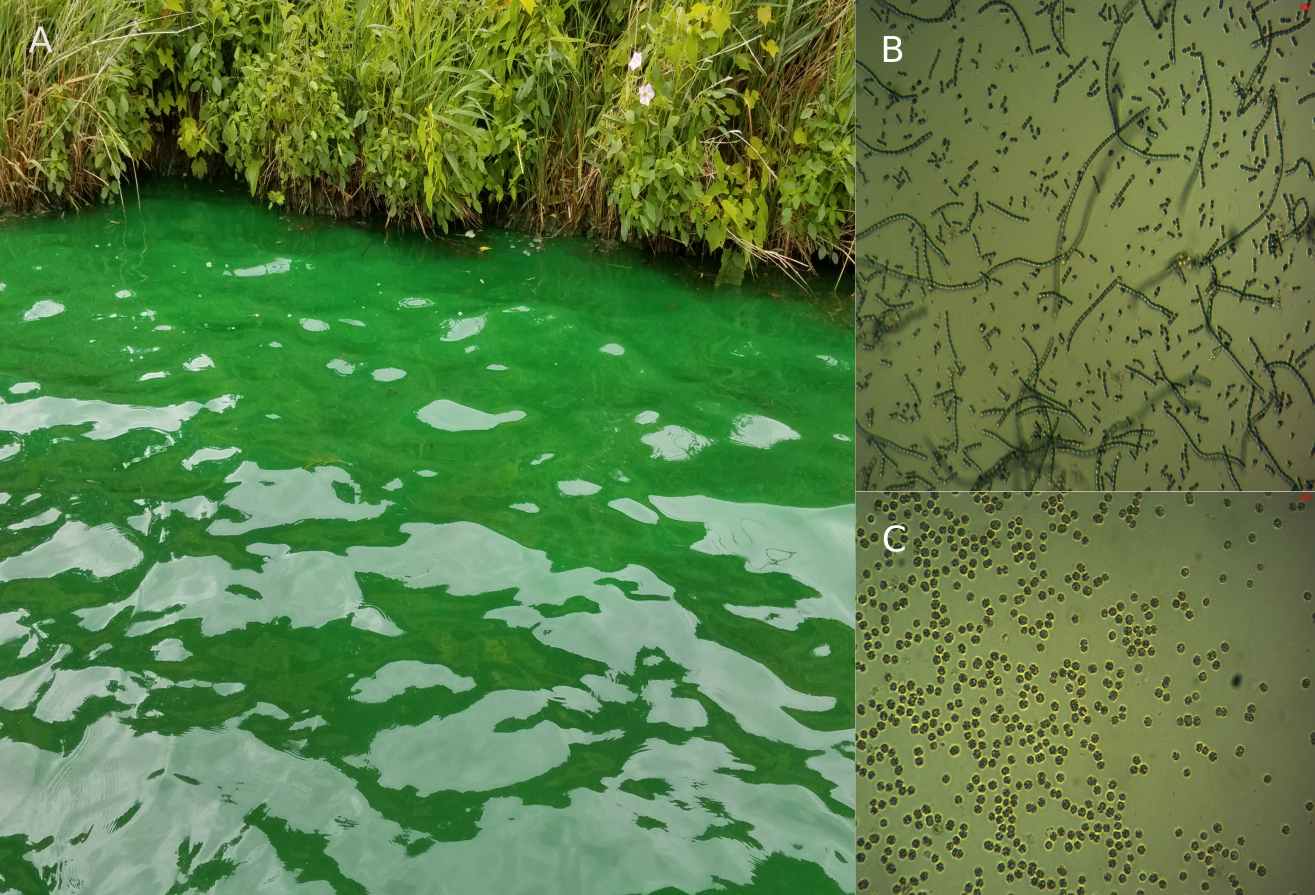
\includegraphics[scale=0.25]{../figures/cyano.png}
	\end{figure}
\end{columns}

\end{frame}
%%%%%%%%%%%%%%%%%%%%%%%%%%%%%%%%%%%%%%%
\begin{frame}{HAB}

	\begin{itemize}
		\item Naturally occuring
		\item Exacerbate from anthropogenic causes \footcite{rastogi_cyanotoxin-microcystins:_2014}
		\item Worldwide issue
		\item Coastal environments
		\item Freshwater lakes
	\end{itemize}

\end{frame}
%%%%%%%%%%%%%%
\begin{frame}{Lake Erie 2014}
	\begin{figure}
		\centering
		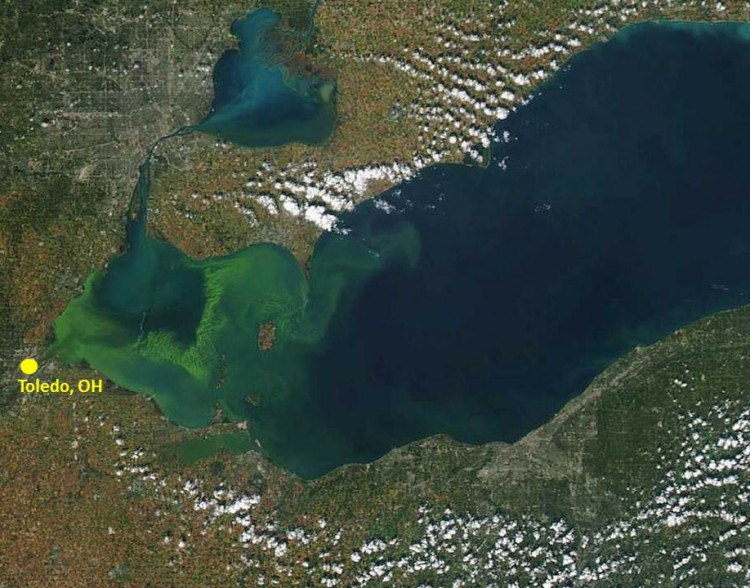
\includegraphics[scale=0.35]{erie.jpg}
	\end{figure}
\hrule
{\tiny cdn.coastalscience.noaa.gov}
\end{frame}
%%%%%%%%%%%%%%
\begin{frame}{Possible causes}

\end{frame}
%%%%%%%%%%%%%%
\begin{frame}{Toxicity}

	\begin{itemize}
		\item Irritant
			\begin{itemize}
				\item Lipolysacharides\footcite{moore_richard_cyanobacterial_1993}
			\end{itemize}
		\item Toxins
			\begin{itemize} 
				\item Microcystin and nodularin \textsuperscript{1}
  				\item Cylindrospermopsin \footcite{dittmann_cyanobacterial_2012}
				\item Anatoxin \footcite{codd_cyanobacterial_1999}
				\item Saxitoxin \textsuperscript{1}
			\end{itemize}
	\end{itemize}

\end{frame}
%%%%%%%%%%%%%%
\begin{frame}{Microcystin}

\begin{columns}
	\column{0.5\textwidth}

	\begin{itemize}
		\item Cyclic peptide
		\item 1000 Da
		\item Hepatoxin and carcinogenic
		\item Inhibits protein phosphatase
		\item Diverse structures

	\end{itemize}
\column{0.5\textwidth}

\begin{figure}
	\centering
	\hspace*{-3cm}
	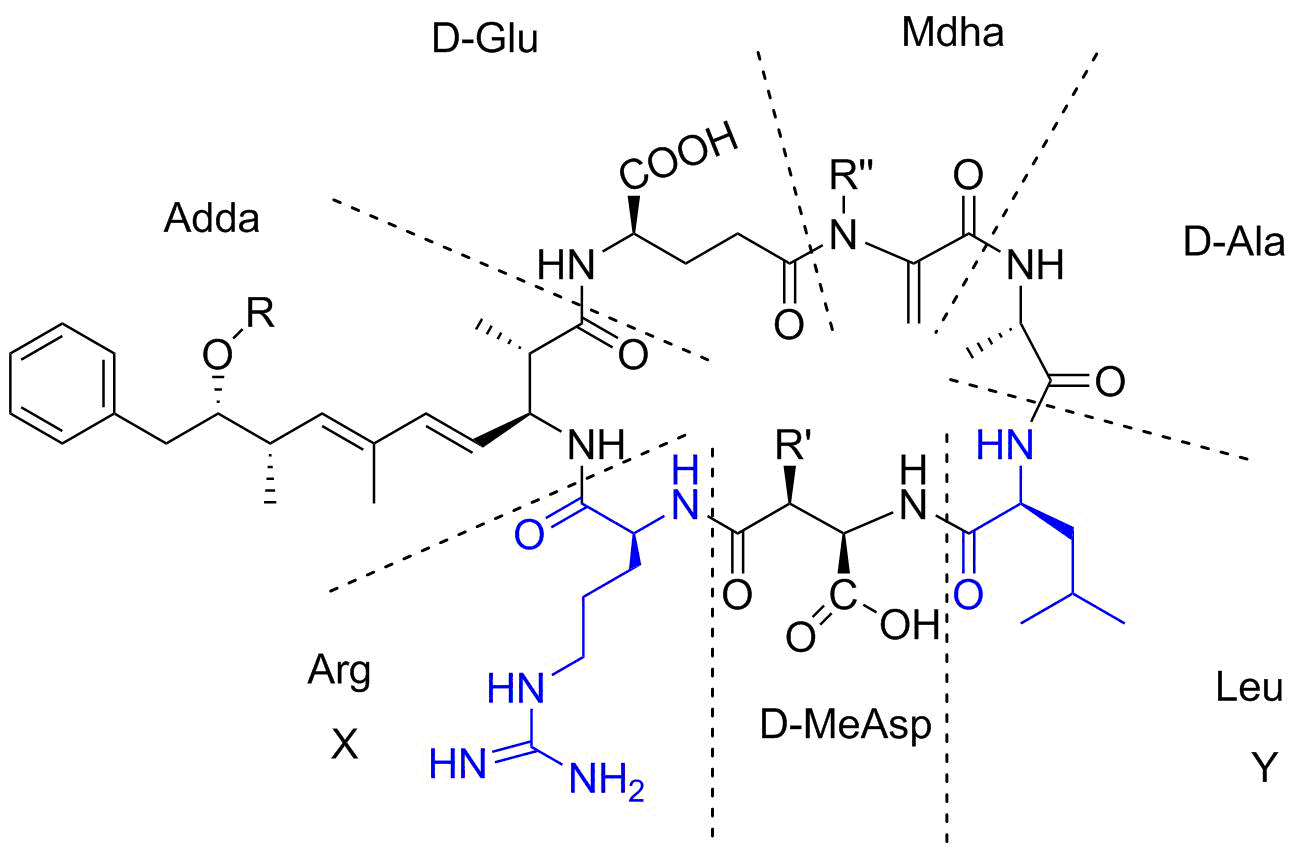
\includegraphics[scale=0.2]{../figures/Microcystin-LR.png}
\end{figure}
\end{columns}

\end{frame}
%%%%%%%%%%%%%%
\begin{frame}{Cylindrospermopsin}
	\begin{itemize}
		\item Polycyclic uracil derivative 
		\item Covalently binds to DNA/RNA 
		\item Inhibits protein synthesis 
		\item  
	\end{itemize}

	<++>
\end{frame}
%%%%%%%%%%%%%%
\begin{frame}{Anatoxin}

\end{frame}
%%%%%%%%%%%%%%
\begin{frame}{Saxitoxin}

\end{frame}
%%%%%%%%%%%%%%
\begin{frame}{Exposure Route}

	\begin{itemize}
		\item Direct contact
		\item Aerosols
		\item Ingestion
		\begin{itemize}
			\item Seafood/Fish 
			\item Drinking water
			\item Algal supplements
		\end{itemize}
	\end{itemize}

\end{frame}
%%%%%%%%%%%%%%
\begin{frame}{Law and Regulation}

	\begin{itemize}
		\item Safe Drinking Water Act
		\item Maximum Contaminant Level
		\begin{itemize}
			\item Regulated and enforced
		\end{itemize}
		\item Contaminant Candidate List
		\begin{itemize}
			\item ``More like guidelines''
		\end{itemize}
	\end{itemize}
\end{frame}
%%%%%%%%%%%%%%
\begin{frame}{Objectives}

\end{frame}
%%%%%%%%%%%%%%
\section{Survey}
\begin{frame}{Surveyed Lakes}

\begin{figure}
	\centering
	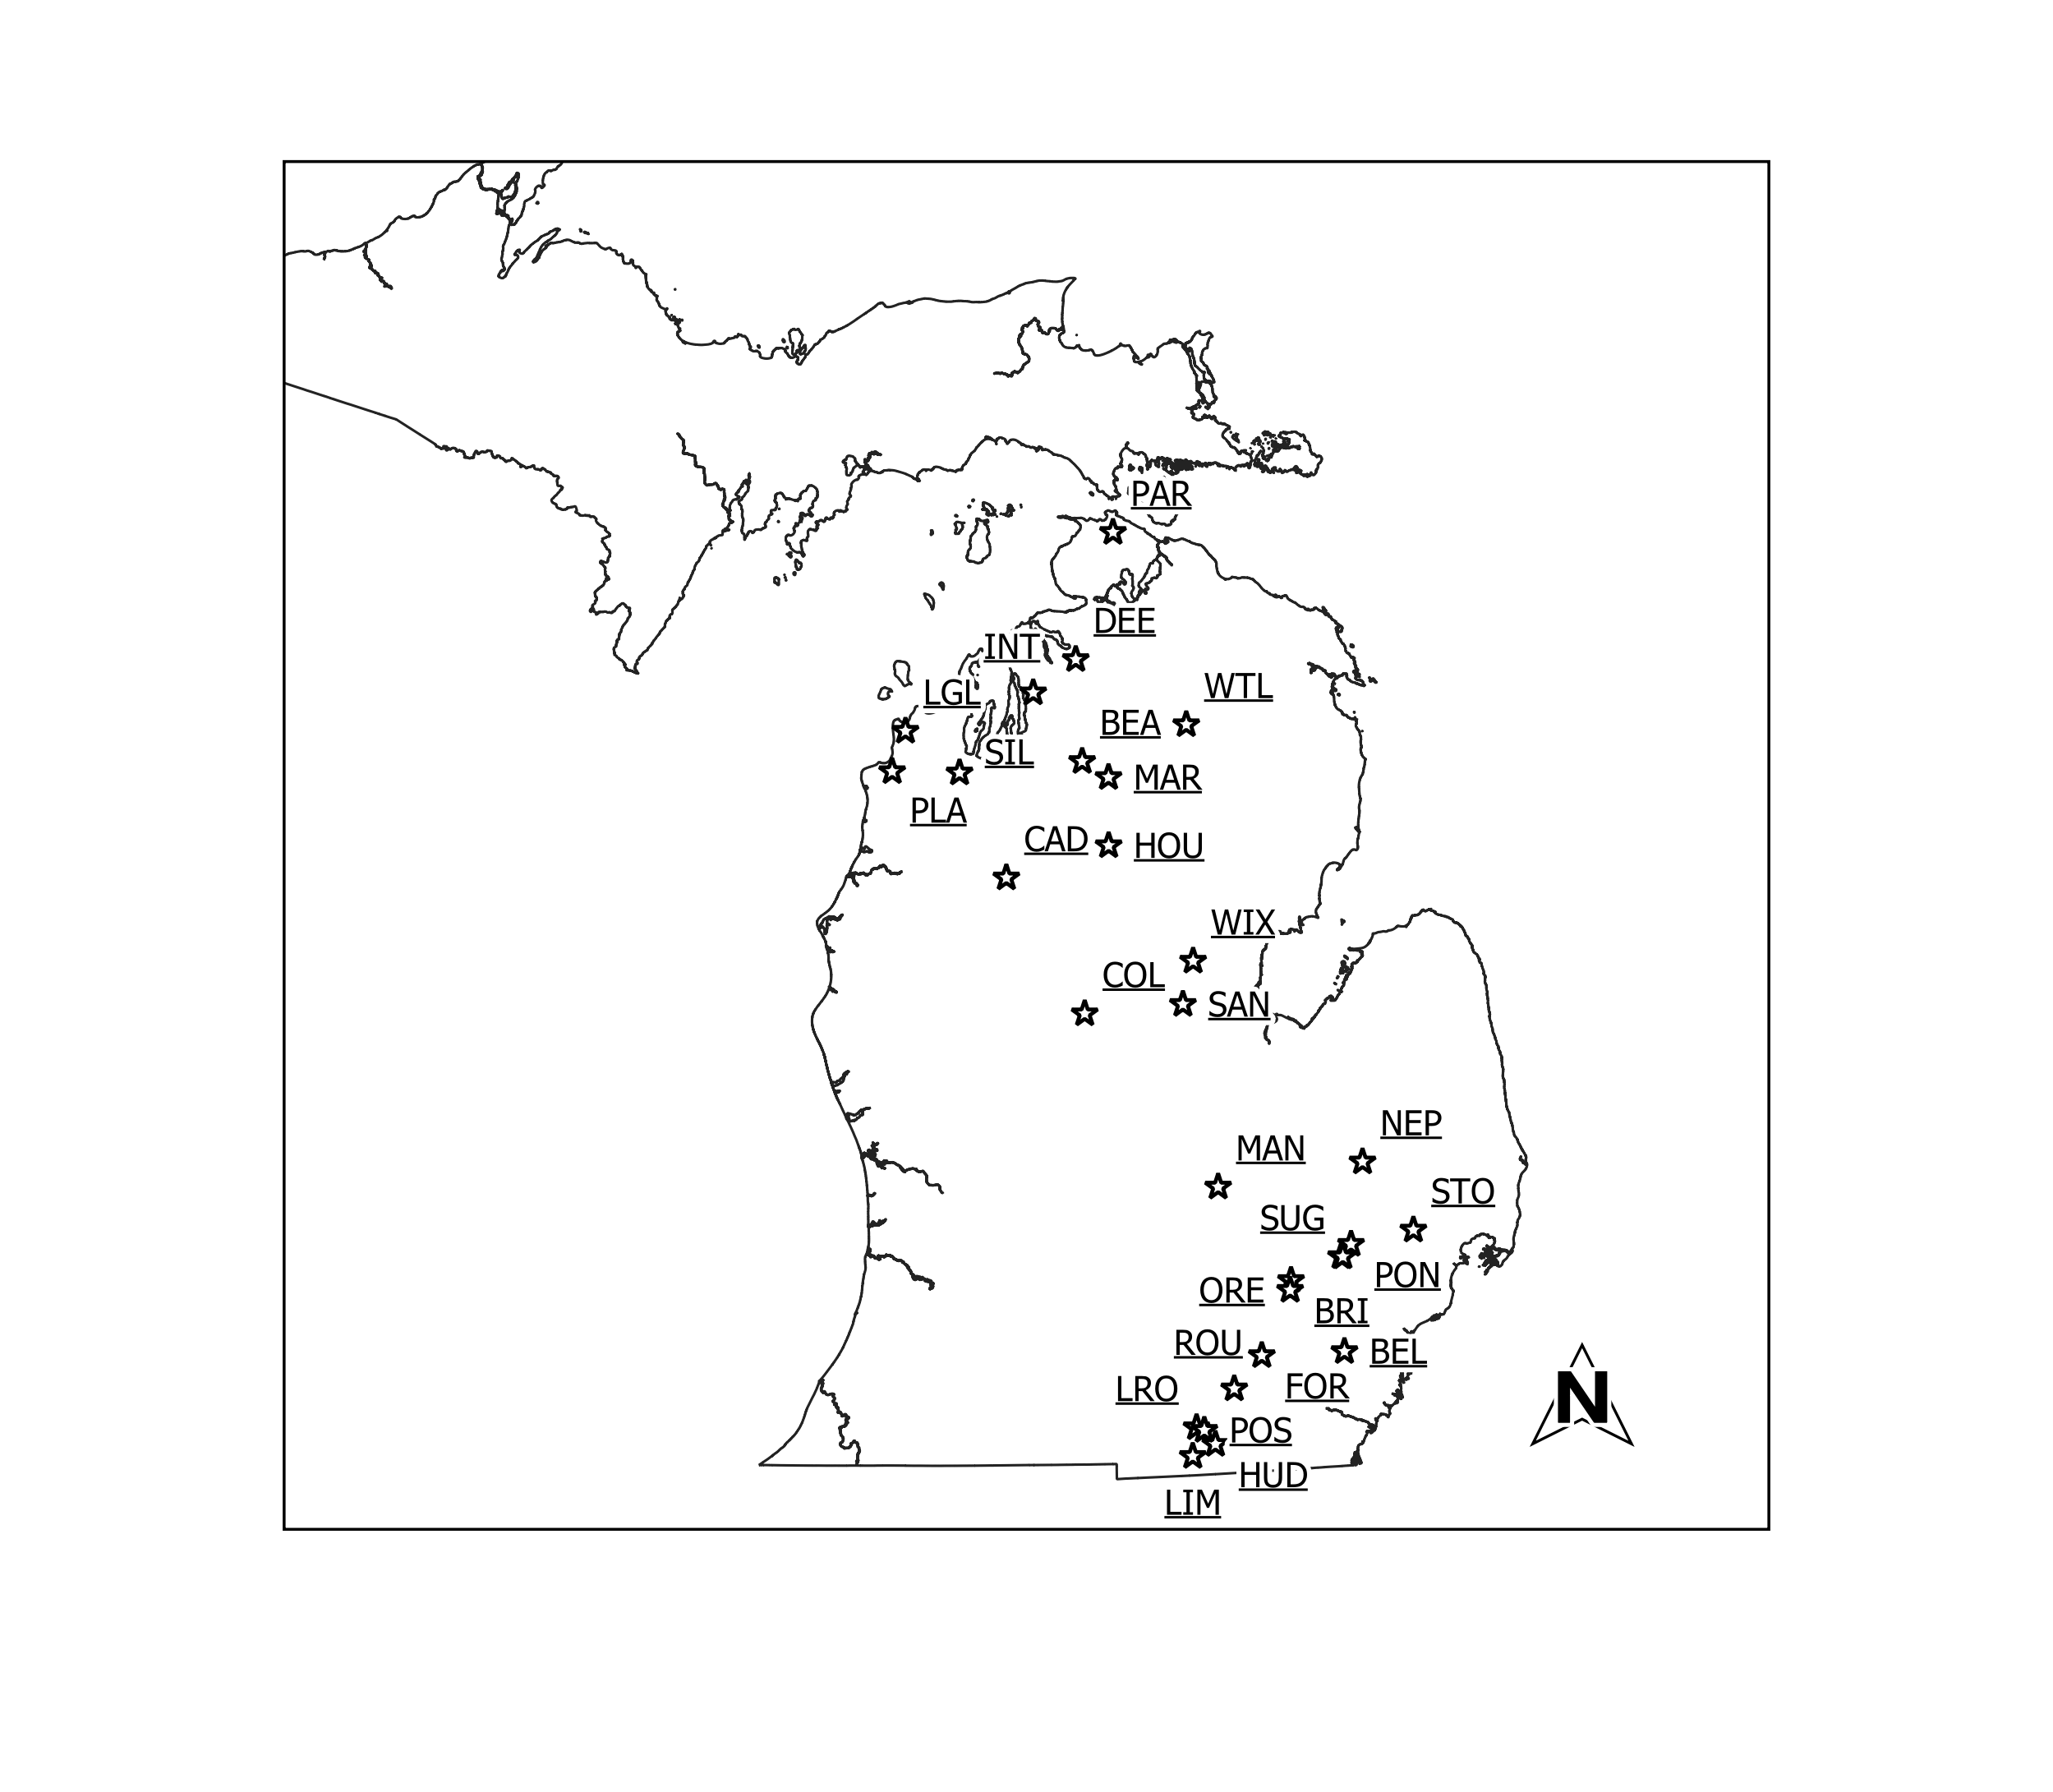
\includegraphics[width=0.8\textwidth,height=\textheight]{../figures/Overview.png}
	\caption{Sampled Lakes}
\end{figure}

\end{frame}

%%%%%%%%%%%%%%%%%%%%%%%%%%
\begin{frame}{Water Sampling}

	\begin{itemize}
		\item Sampled each lake once a month
		\item Collected water
		\item Quickly transported back
		\item Analyzed ASAP
	\end{itemize}

\end{frame}

%%%%%%%%%%%%%%%%%%%%%%%%%%%%%%
\begin{frame}{SPATT}

\begin{columns}
\column{0.5\textwidth}
	\begin{itemize}
		\item Solid phase adsorbtion toxin tracking
		\item Sachet filled with resin
		\item Left for one month
	\end{itemize}

\column{0.5\textwidth}

	\begin{itemize}
		\item test
	\end{itemize}
\end{columns}

\end{frame}

%%%%%%%%%%%%%%%%%%%%%%%%%%%%%
\begin{frame}{Analysis}

\end{frame}

%%%%%%%%%%%%%%%%%%%%%%%%%%%%%%%
\begin{frame}{Nutrients}
	\begin{itemize}
		\item Orthophosphate-P 
		\item Nitrate+nitrite-N
		\item Ammonia-N 
		\item Total Kejdlahl nitrogen 
		\item Total Phosphorus
	\end{itemize}

	<++>

\end{frame}

%%%%%%%%%%%%%%%%%%%%%%%%%%%%%%
\begin{frame}{LC-MS/MS}
	\begin{itemize}
		\item Freeze/Thaw
		\item Filter
	\end{itemize}

\end{frame}

%%%%%%%%%%%%%%%%%%%%%%%%%%%%%
\begin{frame}{SPATT}

	\begin{itemize}
		\item Solid phase adsorbtion toxin tracking
		\item Similiar to the stationary phase
	\end{itemize}

\end{frame}
%%%%%%%%%%%%%%%%%%%%%%%%%%%%%
\begin{frame}{ELISA}

\end{frame}

%%%%%%%%%%%%%%%%%%%%%%%%%%%%%
\begin{frame}{Geospatial Analysis}

\end{frame}
%%%%%%%%%%%%%%%%%%%%%%%%%%%%%
\begin{frame}{Results}

\end{frame}
%%%%%%%%%%%%%%%%%%%%%%%%%%%%%
\begin{frame}{Could we predict HABs?}

\end{frame}

%%%%%%%%%%%%%%%%%%%%%%%%%%%%%
\begin{frame}{Acknowledgment}

	\begin{itemize}
		\item My lab partners Brian Spies and Andrew Herrpich
		\item Jason Sckrabulis, Ryan Mcwhinnie, Melissa Ostrowski
		\item Dr.David Szlag and Dr. Thomas Raffel
		\item Michigan Department Environmental Quality
		\item Oakland University and the Chemistry Department
	\end{itemize}

\end{frame}
